\section{Algorithms}
In recent years, methods of meta learning have emerged one after another. Previous% [77], [78]
categorizations of meta-learning methods tend to produce a three-way taxonomy across optimization-based methods, model-based (or black box) methods, and metric-based (or non-parametric) methods.
Today we mainly introduce the most famous example of optimization-based methods, MAML, which is to learn a good initialization for the parameters, and then use a small amount of updates to train new tasks on the basis of this initialization.

\subsection{MAML}
According to the above introduction, we can realize that: From a macro perspective, meta learning uses tasks as ``samples" for learning! So in general, we will divide the data into $Meta\_train$ and $Meta\_test$, where $Meta\_train$ contains data from multiple tasks, and can be divided into $D\_train$ and $D\_test$, which are used for training and testing respectively.

Since current machine learning methods all perform gradient updates, and the focus of MAML is on gradient updates, it can also be regarded as a gradient-based meta learning method.

The core idea of MAML is actually very simple. In each iteration step, there will be an initial parameter $\theta$, which is used to update the gradient of $K$ tasks in $D\_train$ and achieve new $\theta'_i$ of different tasks. After all $\theta'_i$ optimized on $D\_train$, we update the global parameter $\theta$ on K tasks in $D\_test$(see Figure~\ref{fig:graph}).

\begin{figure}[h]
  \centering
  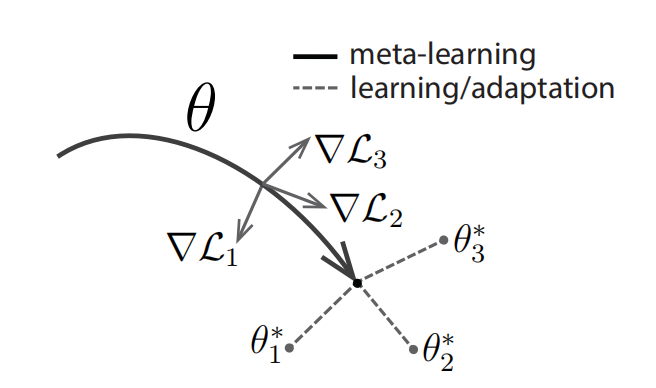
\includegraphics[totalheight=1.5in]{fig1.png}
  \caption{Diagram of our model-agnostic meta-learning algorithm (MAML)} \label{fig:graph}
\end{figure}

The gray branch lines in the figure represent the update direction of $\theta$ on different tasks, and the black line represents the final optimization of the model parameters, which can prevent the parameters from overfitting on a certain task. The last dotted lines represent processes of adaptation to new tasks, which is referred to as the fine-tune of the model parameters.

\begin{algorithm}
  \caption{Model-Agnostic Meta-Learning}
  \label{MAML}
  \begin{algorithmic}[1]
    \REQUIRE $p(\mathcal{T})$: distribution over tasks
    \REQUIRE $\alpha, \beta$: step size hyperparameters
    \STATE randomly initialize $\theta$
    \WHILE {not done}
    \STATE Sample batch of tasks $\mathcal{T}-i \sim p(\mathcal{T})$
    \FORALL {$\mathcal{T}-i$}
    \STATE Evaluate $\nabla-\theta \mathcal{L}-{\mathcal{T}-i} (f-\theta)$ with respect to $K$ examples
    \STATE Compute adapted parameters with gradient descent: $\theta'-i = \theta - \alpha\nabla-\theta \mathcal{L}-{\mathcal{T}-i} (f-\theta)$
    \ENDFOR
    \STATE Update $\theta \leftarrow \theta - \beta\nabla-\theta \Sigma-{\mathcal{T}-i \sim p(\mathcal{T})}\mathcal{L}-{\mathcal{T}-i} (f-{\theta'-i})$
    \ENDWHILE
  \end{algorithmic}
\end{algorithm}